\chapter{Classical versus Quantum Computing}\label{chap:classical_vs_quantum}

This chapter contrasts classical and quantum computing paradigms, highlighting the fundamental differences in information representation, processing capabilities, and underlying principles, particularly concerning their impact on cryptography.

\section{Fundamental Differences}\label{sec:differences}

The core distinctions arise from leveraging quantum mechanics:

\begin{itemize}
    \item \textbf{Information Units:}
    \begin{itemize}
        \item Classical computers use \textbf{bits}, which can deterministically be either 0 or 1.
        \item Quantum computers use \textbf{qubits}, which can exist in a \textbf{superposition} of $|0\rangle$ and $|1\rangle$ simultaneously ($\alpha|0\rangle + \beta|1\rangle$), allowing representation of exponentially more information.
    \end{itemize}
    \item \textbf{State Space:}
    \begin{itemize}
        \item $n$ classical bits can represent one of $2^n$ possible states at any given time. The state space grows linearly with the number of possible states.
        \item $n$ qubits can represent a superposition of all $2^n$ basis states simultaneously. The dimension of the Hilbert space grows \textbf{exponentially} ($2^n$) with the number of qubits.
    \end{itemize}
    \item \textbf{Core Principles Utilized:}
    \begin{itemize}
        \item Classical computing relies on Boolean algebra and deterministic logic gates.
        \item Quantum computing utilizes \textbf{superposition}, \textbf{entanglement} (non-local correlations between qubits), and \textbf{quantum interference} (probability amplitudes can cancel or reinforce each other) to perform computations.
    \end{itemize}
\end{itemize}

\section{Computational Models}\label{sec:computational_models}

\subsection{Classical Computing}\label{subsec:classical}
Classical computers typically operate based on the von Neumann architecture, processing information sequentially using deterministic logic gates. The state of an $n$-bit register is described by a single $n$-bit string, representing one specific state out of $N_{\text{states}} = 2^n$.
\begin{equation}\label{eq:classical_states_ch4}
    \text{Classical State Space Size} = 2^n
\end{equation}
Algorithms are designed based on sequential or parallel execution of classical logic operations.

\subsection{Quantum Computing}\label{subsec:quantum}
Quantum computers manipulate qubits using quantum gates (unitary transformations). An $n$-qubit system's state is described by a vector $|\psi\rangle$ in a $2^n$-dimensional complex Hilbert space:
\begin{equation}\label{eq:quantum_state_ch4}
    |\psi\rangle = \sum_{i=0}^{2^n-1} \alpha_i|i\rangle
\end{equation}
where $|i\rangle$ represents the $i$-th computational basis state (an $n$-qubit binary string), and $\alpha_i$ are complex probability amplitudes satisfying $\sum_{i=0}^{2^n-1} |\alpha_i|^2 = 1$.

\textbf{Quantum Parallelism vs Classical Parallelism:} While superposition allows a quantum computer to compute on all $2^n$ basis states simultaneously in some sense ("quantum parallelism"), extracting useful information is non-trivial due to the probabilistic nature of quantum measurement. A measurement typically collapses the superposition into a single classical outcome. Quantum algorithms are cleverly designed to use interference to amplify the probability amplitudes of desired outcomes while cancelling others, allowing efficient solutions for specific problems that exploit this structure. This differs significantly from classical parallelism, which involves executing multiple computations simultaneously on different processors.

\section{Computational Complexity Classes}\label{sec:complexity_classes}
Understanding the theoretical power of different computing models involves complexity classes:
\begin{itemize}
    \item \textbf{P (Polynomial time):} Problems solvable by a classical deterministic computer in polynomial time relative to the input size.
    \item \textbf{BPP (Bounded-error Probabilistic Polynomial time):} Problems solvable by a classical probabilistic computer in polynomial time with an error probability bounded below 1/2.
    \item \textbf{BQP (Bounded-error Quantum Polynomial time):} Problems solvable by a quantum computer in polynomial time with an error probability bounded below 1/2.
\end{itemize}
It is strongly believed that $\textbf{P} \subseteq \textbf{BPP} \subseteq \textbf{BQP}$. Shor's algorithm demonstrates that \textbf{Integer Factorization} is in \textbf{BQP}. However, factoring is not known to be in \textbf{BPP} (or \textbf{P}), suggesting that quantum computers may be fundamentally more powerful than classical computers for certain tasks.

\begin{figure}[h]
    \centering
    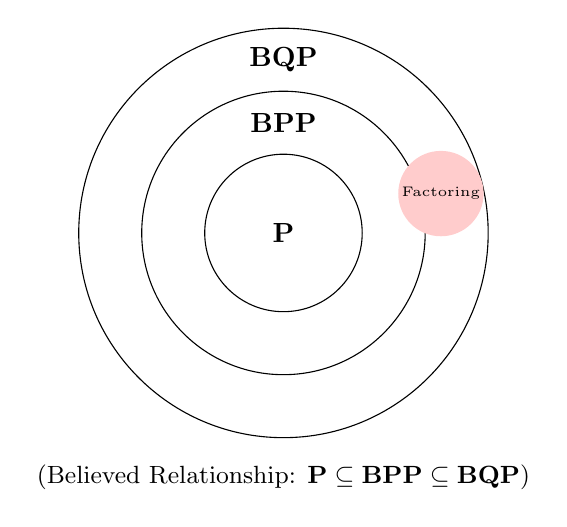
\begin{tikzpicture}
        % Define radii
        \def\radiusP{1.0}
        \def\radiusBPP{1.8}
        \def\radiusBQP{2.6}
        
        % Draw ellipses (approximating sets)
        \draw (0,0) circle (\radiusP);
        \node at (0,0) {\textbf{P}};
        
        \draw (0,0) circle (\radiusBPP);
        \node at (0, \radiusBPP - 0.4) {\textbf{BPP}};
        
        \draw (0,0) circle (\radiusBQP);
        \node at (0, \radiusBQP - 0.4) {\textbf{BQP}};

        % Indicate Factoring
        \node[fill=red!20, circle, inner sep=1pt, font=\tiny] (factoring) at (\radiusBPP + 0.2, 0.5) {Factoring};
        
        % Indicate relationship belief
        \node[font=\small, align=center] at (0, -\radiusBQP - 0.5) {(Believed Relationship: $\textbf{P} \subseteq \textbf{BPP} \subseteq \textbf{BQP}$)};
    \end{tikzpicture}
    \caption{Conceptual relationship between complexity classes P, BPP, and BQP. Factoring is known to be in BQP but is believed to be outside BPP.}
    \label{fig:complexity_classes}
\end{figure}

\section{Processing Power and Cryptographic Impact}\label{sec:processing_and_crypto_impact}

The difference in computational models leads to significant variations in processing power for specific tasks critical to cryptography:

\begin{table}[h]
    \centering
    \caption{Computational Complexity Comparison for Cryptographically Relevant Problems}
    \label{tab:computing_power_ch4}
    \begin{tabular}{@{}lccc@{}}
        \toprule
        \textbf{Operation} & \textbf{Input Size Param.} & \textbf{Classical Complexity} & \textbf{Quantum Complexity} \\
        \midrule
        Integer Factoring & $n = \log N$ (bits) & $O(e^{c n^{1/3}(\log n)^{2/3}})$ & $O(n^2 \log n \log\log n)$ \\
        Database Search & $N$ items & $O(N)$ & $O(\sqrt{N})$ \\
        Matrix Multiplication & $n \times n$ matrix & $O(n^\omega), \omega \approx 2.37$ & $O(n^{2.24})$ \\
        \bottomrule
    \end{tabular}
    \caption*{Note: Classical factoring complexity refers to the General Number Field Sieve (GNFS). Quantum complexities often represent query complexity or gate counts under idealized conditions.}
\end{table}

\textbf{Qualitative Impact on Cryptography:} Quantum computers do not simply speed up all computations uniformly. Their power stems from exploiting specific problem structures:
\begin{itemize}
    \item \textbf{Shor's Algorithm:} Exploits the periodic structure inherent in modular exponentiation (related to factoring and discrete logarithms) using the Quantum Fourier Transform. This yields an \textit{exponential} speedup, breaking current public-key cryptography.
    \item \textbf{Grover's Algorithm:} Provides a \textit{quadratic} speedup for unstructured search problems. This impacts symmetric key ciphers and hash functions by reducing the effective security against brute-force attacks.
\end{itemize}

Key differences in cryptographic applications:
\begin{itemize}
    \item \textbf{Key Generation:}
    \begin{itemize}
        \item Classical: Based on mathematical difficulty
        \item Quantum: Potential for information-theoretic security
    \end{itemize}
    \item \textbf{Encryption Speed:}
    \begin{itemize}
        \item Classical: Efficient for symmetric encryption
        \item Quantum: Potentially faster for specific operations
    \end{itemize}
    \item \textbf{Security Assumptions:}
    \begin{itemize}
        \item Classical: Computational hardness
        \item Quantum: Physical principles
    \end{itemize}
\end{itemize}

\section{Practical Considerations}\label{sec:practical_ch4}

Implementation challenges and considerations:

\begin{itemize}
    \item \textbf{Hardware Requirements:}
    \begin{itemize}
        \item Classical: Mature technology with established manufacturing processes
        \item Quantum: Significant engineering challenges including cryogenic cooling and precise control systems
    \end{itemize}
    \item \textbf{Error Rates:}
    \begin{itemize}
        \item Classical: Highly reliable with negligible error rates
        \item Quantum: Extremely sensitive to noise (decoherence), requiring extensive Quantum Error Correction (QEC). Implementing complex algorithms like Shor's requires thousands or millions of physical qubits to encode a single reliable logical qubit
    \end{itemize}
    \item \textbf{Scalability:}
    \begin{itemize}
        \item Classical: Well-understood scalability principles
        \item Quantum: Major challenges in scaling while maintaining qubit quality and connectivity
    \end{itemize}
\end{itemize}

\section{Future Outlook}\label{sec:outlook_ch4}

The relationship between classical and quantum computing:

\begin{itemize}
    \item \textbf{Complementary Roles:}
    \begin{itemize}
        \item Hybrid algorithms combining quantum and classical components
        \item Specialized applications leveraging quantum advantages
        \item Integration of quantum accelerators with classical systems
    \end{itemize}
    \item \textbf{Development Timeline:}
    \begin{itemize}
        \item Near-term (NISQ era): Focus on demonstrating quantum advantage
        \item Medium-term: Development of early fault-tolerant systems
        \item Long-term: Possibility of large-scale quantum computers capable of running Shor's algorithm
    \end{itemize}
\end{itemize}

This comparison demonstrates the fundamental differences between classical and quantum computing. While quantum computers offer transformative potential for specific computational tasks, including breaking widely used public-key cryptosystems, their practical realization faces substantial challenges related to hardware, error correction, and scalability.